\chapter{系统需求分析}

本章主要围绕基于 MIL-STD-6016 的战术数据链信息标准数据库及其应用平台,分析系统的整体需求,明确功能性与非功能性要求,以便为后续系统设计与实现提供依据。

战术数据链作为现代联合作战的核心通信手段,其信息标准数据库的建设对于提升作战效能、增强系统互操作性具有重要意义。随着网络中心战概念的深入发展和多域作战需求的不断增长,传统的战术数据链系统面临着数据管理复杂、标准版本多样、跨链路互操作困难等挑战。因此,构建一个统一、高效、可扩展的战术数据链信息标准数据库系统,已成为当前军事信息化建设的重要任务。

本章将从系统需求分析的角度,全面阐述基于MIL-STD-6016标准的战术数据链信息标准数据库系统的功能需求、非功能性需求、数据特征与处理需求以及用户角色与交互需求。通过对这些需求的深入分析,为后续的系统架构设计、数据库建模、前后端开发以及系统集成测试提供明确的技术指导和约束条件。

\section{功能需求}

根据前期调研和标准分析,结合实际应用场景,系统需要实现以下核心功能:

\subsection{数据特征与处理需求}
战术数据链消息具有与传统业务数据不同的特性,其处理需求也更为复杂。为保证数据库的适用性与系统的实用性,需从数据来源、结构特征、处理方式与存储管理等角度加以分析\cite{baek2016_jsac}。

系统数据主要来源于 {MIL-STD-6016}、{MIL-STD-3011}、{STANAG-5516} 等标准文档,并结合 {MAVLink}、{NMEA-0183}、{ARINC-429} 等协议数据。数据类型主要包括:

(1)标准消息数据:J 系列报文(J2.0、J3.0、J7.0、J12.0等)及其字段定义;

(2)语义概念数据:基于CDM四层法的概念库和字段映射关系;

(3)多格式文档数据:PDF、XML、JSON、CSV等格式的标准文档和配置文件;

(4)跨协议转换数据:不同协议间的消息转换和映射规则。

表\ref{table_data_features}详细展示了战术数据链数据特征与处理需求的对应关系,该表从数据类型、结构特点、处理需求和存储实体四个维度进行了系统性的分析。

\begin{table}[!htb]
    \caption{战术数据链数据特征与处理需求概览}
    \label{table_data_features}
    \centering
    \adjustbox{width=0.9\textwidth,center}{%
    \begin{tabular}{lccc}
        \hline
        \textbf{数据类型} & \textbf{结构特点} & \textbf{处理需求} & \textbf{存储实体} \\
        \hline
        标准消息数据 & 多字段/比特位 & 报文解析、完整性校验 & 消息表、字段表 \\
        语义概念数据 & 概念层次/同义映射 & 概念绑定、语义一致性 & 概念表、绑定表 \\
        多格式文档数据 & 格式多样/结构复杂 & 多格式解析、智能识别 & 文档表、解析结果表 \\
        跨协议转换数据 & 格式差异/协议适配 & 格式转换、协议映射 & 映射表、转换规则表 \\
        \hline
    \end{tabular}%
    }
\end{table}


\subsection{标准消息管理}
战术数据链信息标准数据库系统需要支持多种消息标准的统一管理\cite{CurtissWright_TCG_HUNTR_2020}。根据实际应用需求分析,系统应具备以下核心能力:

(1)多标准消息支持:系统需要同时支持MIL-STD-6016的J系列消息(J2.0、J3.0、J7.0、J12.0等)、MAVLink的飞行器通信消息(HEARTBEAT、ATTITUDE、POSITION等)、NMEA-0183的导航消息(GGA、RMC、VTG等)等多种标准。每种消息标准都有其特定的格式、语义和应用场景,系统需要能够完整地存储和管理这些消息的定义信息,包括消息的基本属性、消息结构以及消息的语义信息。

下表\ref{table_supported_standards}详细列出了系统需要支持的主要标准和协议。

\begin{table}[!htb]
    \caption{系统支持的标准和协议}
    \label{table_supported_standards}
    \centering
    \adjustbox{width=0.9\textwidth,center}{%
    \begin{tabular}{lccc}
        \hline
        \textbf{标准名称} & \textbf{描述} & \textbf{版本} & \textbf{主要消息类型} \\
        \hline
        MIL-STD-6016 & 美军标准6016 - 战术数据链消息标准 & A, B, C & J2.0, J3.0, J7.0, J12.0, J13.0 \\
        MIL-STD-3011 & 美军标准3011 - 联合战术信息分发系统 & A, B & J2.0, J2.2, J3.0, J3.1, J3.3 \\
        STANAG-5516 & 北约标准5516 - 战术数据交换 & 1, 2, 3 & J2.0, J3.0, J7.0, J12.0 \\
        MAVLink & 微型飞行器通信协议 & 1.0, 2.0 & HEARTBEAT, ATTITUDE, POSITION, GPS\_RAW\_INT \\
        NMEA-0183 & 海洋电子设备数据格式 & 2.0, 2.1, 2.2, 2.3 & GGA, RMC, VTG, GLL, GSA \\
        ARINC-429 & 航空电子设备数字信息传输 & 15, 16, 17 & A429, A629 \\
        \hline
    \end{tabular}%
    }
\end{table}

(2)消息录入与维护:考虑到标准文档的复杂性和多样性,系统需要支持多种数据录入方式。传统的逐条录入方式效率低下,无法满足大规模标准文档的处理需求。系统需要提供基于PDF文档的自动化解析功能,能够从标准文档中自动提取消息定义信息,并支持CSV、Excel、XML、JSON等多种格式的批量导入和单个录入两种方式。

(3)消息字段管理:J系列消息的字段结构复杂,包含字段名称、起始位置、结束位置、位长度、描述信息等多个属性。系统需要能够处理这种复杂的字段结构,并建立字段与消息之间的关联关系。同时,系统需要支持字段的层次化组织,如字段组、子字段等,以便于更好地管理和理解消息结构。


\subsection{字段与语义概念绑定}
为提升消息语义一致性,系统需要支持字段与语义概念的绑定\cite{Chelton_Link16_Antennas_2022}。根据实际应用需求分析,系统应具备以下核心能力:

(1)语义概念库构建:需建立统一的语义概念库,包含战术数据链领域中的核心概念,如平台标识、位置信息、时间信息、任务状态等。每个语义概念都应具有明确的定义、属性描述和使用规则,支持概念的层次化组织和继承关系。

(2)字段绑定机制:系统需要支持自动绑定和手动绑定两种方式。自动绑定基于字段名称、数据类型、取值范围等特征进行匹配,能够快速建立初步的绑定关系。手动绑定允许专家用户根据领域知识进行精确的绑定操作,确保绑定的准确性和完整性。

(3)置信度管理:在功能上需要为每个字段-概念绑定关系分配置信度值,反映绑定的可靠程度。置信度可以通过字段名称相似度、数据类型匹配度、专家验证结果等因素计算,并提供置信度阈值设置功能,允许用户根据应用需求调整绑定标准。

(4)动态绑定更新:考虑到战术数据链标准的不断演进,应支持语义绑定的动态更新,当标准版本更新或新增消息类型时,能够自动检测需要重新绑定的字段,并提供批量更新功能。

\subsection{多链路互操作支持}
考虑到战术数据链存在多标准并行的情况,系统需要具备跨链路的互操作支持功能\cite{AFCEA_Link16_Improvements_2022}。根据实际应用需求分析,系统应具备以下核心能力:

(1)CDM四层法架构:系统需采用CDM(Common Data Model)四层法架构实现多协议互操作。概念层定义统一的语义概念库,包含作战实体、态势要素、指挥关系等核心概念;映射层通过声明式规则定义协议间的字段映射关系;转换层实现具体的消息转换逻辑;运行层提供协议中介和转换引擎。系统支持MIL-STD-6016、MAVLink、MQTT、NMEA-0183等协议的互操作转换,这种分层架构确保系统的可扩展性和可维护性。

图\ref{fig_cdm_architecture}展示了CDM四层法架构,包括语义层(统一概念库)、映射层(YAML配置规则)、校验层(一致性验证)和运行层(转换引擎),展现了多协议间的语义互操作和实时转换。

\begin{figure}[H]
    \centering
    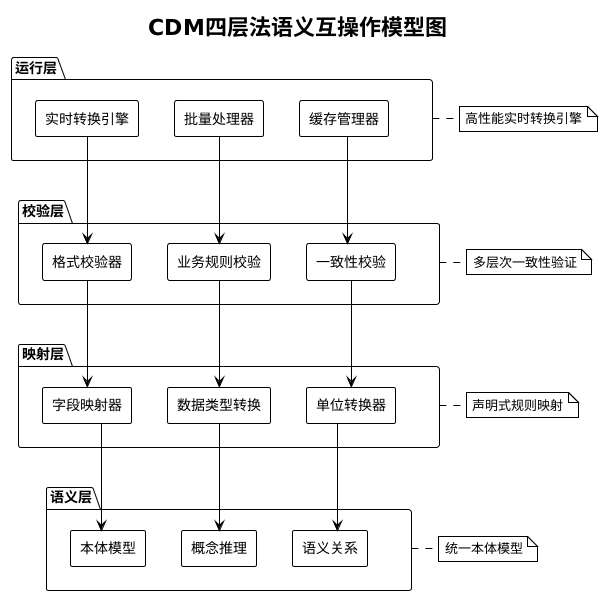
\includegraphics[width=0.6\textwidth,height=0.5\textheight,keepaspectratio]{chapters/fig-0/cdm_four_layer_simple.png}
    \caption{CDM四层法架构图}
    \label{fig_cdm_architecture}
\end{figure}

(2)智能消息转换引擎:应实现基于规则和机器学习的智能转换引擎,能够自动处理协议间的语法差异、语义差异和时序差异。转换引擎需要支持多种转换策略,包括精确匹配、模糊匹配、语义推理等,并提供转换质量评估和置信度评分机制。

(3)统一API网关:需提供统一的API网关,支持多种协议的消息转换和路由。网关需要集成CDM四层法和语义互操作两种处理方式,能够根据源协议和目标协议自动选择最优的转换策略。
下表\ref{table_api_interfaces}列出了系统提供的5个主要API接口及其功能,通过RESTful架构设计为前端界面和外部系统提供标准化数据交换接口。

\begin{table}[!htb]
    \caption{系统API接口功能表}
    \label{table_api_interfaces}
    \centering
    \adjustbox{width=0.9\textwidth,center}{%
    \begin{tabular}{lccc}
        \hline
        \textbf{API接口} & \textbf{主要功能} & \textbf{支持格式} & \textbf{应用场景} \\
        \hline
        /api/v2 & 消息转换、概念管理、映射管理、系统统计 & JSON, XML & 统一文档处理与语义互操作 \\
        /api/cdm & CDM概念创建、映射规则管理、消息转换 & JSON, YAML & CDM四层法互操作处理 \\
        /api/semantic & 语义字段管理、消息映射、路由处理 & JSON, XML & 语义互操作系统 \\
        /api/pdf & PDF文档解析、表格提取、数据处理 & PDF, JSON & MIL-STD-6016文档处理 \\
        /api/mqtt & MQTT消息处理、协议转换、数据路由 & JSON, MQTT & MQTT协议消息处理 \\
        \hline
    \end{tabular}%
    }
\end{table}

(4)协议适配支持:功能设计上应支持MIL-STD-6016、MAVLink、MQTT、NMEA-0183、ARINC-429等多种协议的消息对接,能够处理不同协议间的消息格式差异、语义差异和时序差异。通过声明式映射规则和版本治理机制,系统需要能够灵活应对协议演进和标准更新。


\subsection{前端交互与可视化}
基于前述数据库操作与维护的需求,战术数据链信息标准数据库系统面向的用户群体包括系统管理员、作战指挥员、研发人员等,这些用户具有不同的技术背景和使用需求,因此前端系统应具备以下核心能力:

(1)统一用户界面:需提供统一文档处理与语义互操作平台,包含消息处理、文件处理、概念管理、映射管理、系统概览等核心功能模块,支持用户通过消息号、字段名、J系列类别、时间范围等多种条件进行精确查询,并支持查询条件的保存和重用,允许用户创建常用的查询模板。

(2)数据展示与搜索:应支持多种数据展示方式,包括表格、图表、关系图等,其中表格展示需支持排序、筛选、分页等功能,并提供数据导出能力,图表展示应支持多种图表类型,如柱状图、饼图、折线图等,帮助用户直观地理解数据分布和趋势。同时,系统还应提供智能搜索功能,支持模糊匹配和语义搜索,帮助用户快速定位所需信息。

(3)交互式操作:为确保良好的用户体验和系统可用性,需支持交互式操作和响应式设计。系统应支持拖拽、点击、缩放等交互操作,允许用户通过直观的手势操作来浏览和操作数据,并提供上下文菜单、快捷键等便捷操作方式,提高用户的操作效率。

系统需针对不同用户提供差异化的交互模式\cite{reid_2018_nav_leo}:

(1)图形化交互:前端界面提供消息检索、态势展示和跨链协议映射的可视化操作,支持CDM互操作接口、语义互操作接口和统一处理器接口,降低使用门槛,如图\ref{fig_usecase_frontend}所示。
% ================= 新增:用例图 =================
\begin{figure}[H]
    \centering
    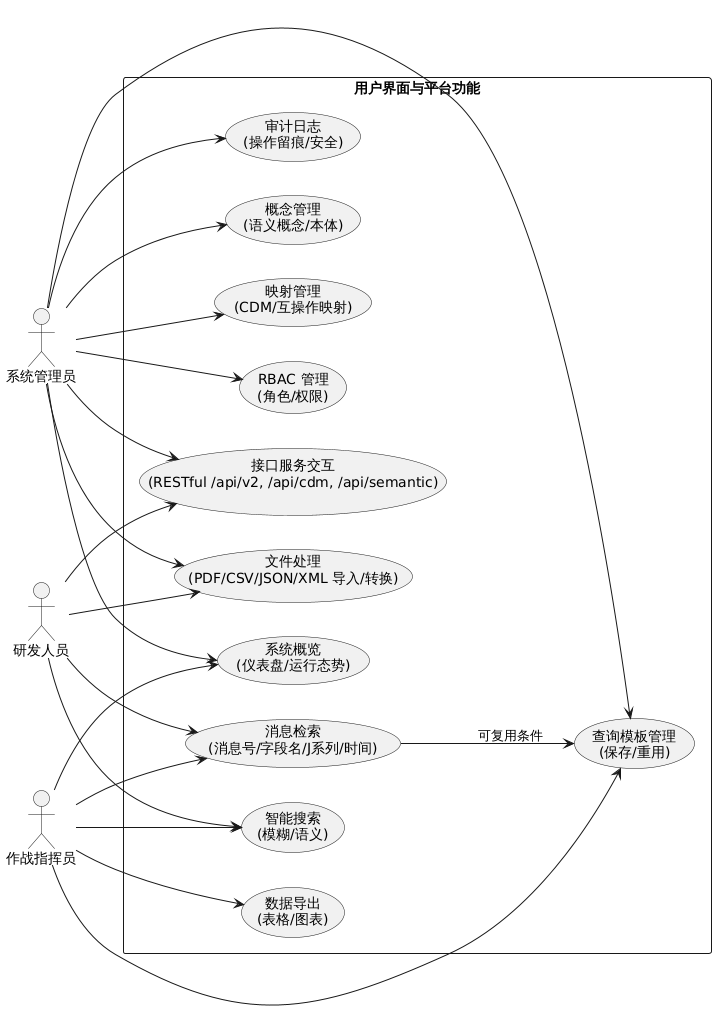
\includegraphics[width=0.8\textwidth,height=0.5\textheight,keepaspectratio]{chapters/fig-0/usecase_frontend.png}
    \caption{前端交互用例图(角色与功能关系)}
    \label{fig_usecase_frontend}
  \end{figure}
(2)命令行接口:为研发与仿真人员提供批处理与脚本化调用,支持大规模数据处理与自动化测试。

(3)接口服务交互:通过 RESTful API 与外部仿真平台或作战系统对接,支持标准化协议调用和跨域互操作,提供/api/v2、/api/cdm、/api/semantic等统一API接口,如图\ref{fig_component_frontend} 所示。



% ================= 新增:组件图 =================
\begin{figure}[H]
  \centering
  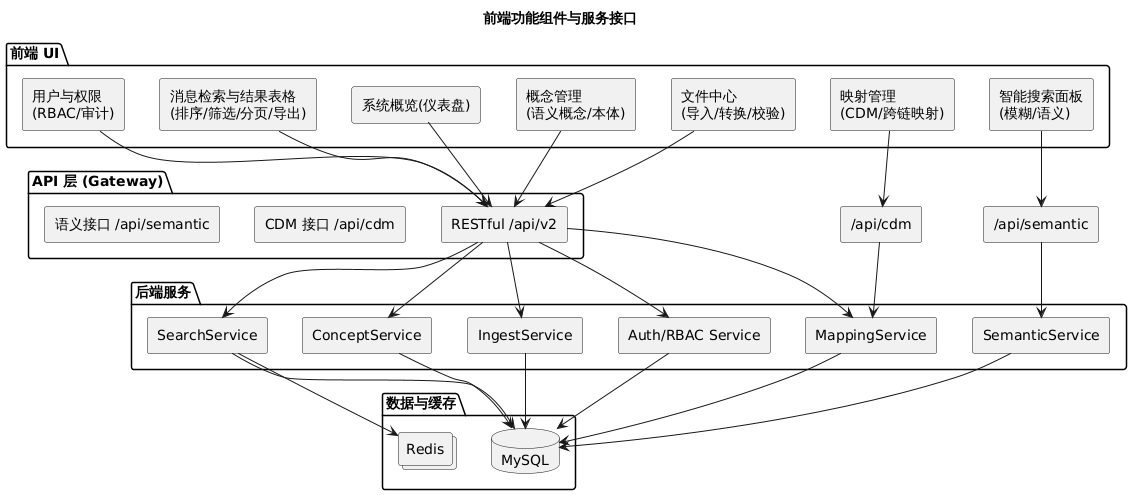
\includegraphics[width=0.8\textwidth,height=0.6\textheight,keepaspectratio]{chapters/fig-0/component_frontend.png}
  \caption{前端功能组件与服务接口关系图}
  \label{fig_component_frontend}
\end{figure}


\subsection{仿真与验证接口}
战术数据链系统的验证与测试依赖于高质量的仿真数据支撑,而仿真平台的有效运行则需要准确的消息定义和格式规范作为基础。基于这一需求,系统必须构建完善的仿真与验证接口体系。

而在面向接口设计时,系统应采用标准化的RESTful API架构,为仿真平台提供数据查询、消息生成、结果验证等核心功能。接口实现严格遵循REST架构原则,采用标准HTTP方法和状态码,确保接口的易用性和可维护性。同时,系统支持多种标准化消息输出格式(JSON、XML、YAML),满足不同仿真平台的格式需求。消息格式包含完整的定义信息,涵盖消息结构、字段定义、语义信息等关键要素,保障仿真平台对消息数据的准确理解和处理。

\section{系统非功能性需求分析}

战术数据链数据库及应用平台作为支撑作战指挥的关键信息系统,除了满足功能性需求外,还必须具备良好的非功能性特征,包括性能、安全性、可扩展性等方面的要求,以确保系统在复杂作战环境下的稳定运行和长期发展\cite{Kagioglidis_2009}。

\subsection{性能需求}
基于战术数据链系统的实时性特征和作战指挥的时效性要求,系统性能需求分析应从响应时间、数据吞吐量和系统可靠性三个维度进行考量\cite{Kee_2008,baek2016_adhoc,baek2019_jsyst_timemirror}。响应时间需求分析表明,多用户并发访问场景和实时态势更新的业务需求对系统响应性能提出了严格要求。通过分析战术数据链消息解析与字段检索的快速响应要求,可以确定普通查询请求的平均响应时间应控制在2秒以内,这一指标直接影响作战指挥的决策效率。为满足上述性能要求,系统需要实现缓存机制,包括Redis缓存和查询结果缓存,对于频繁访问的消息类型和字段定义实现预加载策略,同时建立数据库索引支持多条件组合查询的快速执行。

而对于数据吞吐量的需求,则决定了系统需要处理大规模批量数据导入导出操作,以支撑标准文档的批量处理和系统初始化需求。通过分析仿真测试场景的数据处理需求,可以确定仿真接口应具备持续处理高并发消息流的能力,实现消息的实时生成与回放功能,满足大规模仿真测试的数据处理需求\cite{lee2018_jsyst,Spyridis_2010,Kopp_Throughput_Enhanced_JTIDS_2006,Juarez_2025}。系统可靠性需求分析表明,战术环境的复杂性和不确定性对系统容错能力和数据完整性保障提出了严格要求。通过分析数据安全性和一致性要求,可以确定数据库应具备备份与日志恢复能力,确保数据在异常情况下的安全性。同时,消息存储与语义绑定过程的事务一致性约束需求进一步强化了对系统可靠性的要求,以避免数据不一致问题\cite{Koromilas_2009,EverythingRF_STT}。

\subsection{安全性需求}
战术数据链系统涉及敏感作战信息,安全性需求至关重要。系统必须在数据存储、传输与访问控制等方面提供基本的安全保障,以确保信息不被篡改、泄露或非法利用\cite{Collins_TTNT_immersion_2020}。系统应在数据存储和传输过程中采用加密技术,数据库层面应对核心字段进行加密存储,系统接口需采用基于TLS/SSL的安全传输协议,防止中间人攻击,消息交互采用密钥管理机制,定期更新密钥,防止密钥泄露\cite{Euromids_2025_contract}。

为防止非法访问与误操作,需要建立访问控制机制,提供基于角色的访问控制(RBAC),不同用户角色具备不同权限范围,对数据库的读写操作需进行身份认证与授权,提供日志审计功能,记录用户操作轨迹,便于事后追溯\cite{GovConWire_Euromids_2025}。系统应提供数据校验与完整性验证机制(如哈希校验),在通信中断或错误发生时,系统可通过重传机制与数据恢复策略保证一致性\cite{musumeci_2014_ietrsn_pulseblank,borio_2013_ietspr_pulseblanking,houdzoumis2009_jn,wu_2016_taes_dme_wp,huo_2015_ieeecl_meb,huo_2015_comex_mixed_interference,mitch_2016_nav_chirp_geolocation,vandermerwe_2023_nav_mpanf}。

\subsection{可扩展性需求}
基于战术数据链标准的不断更新与作战样式的演进趋势,系统可扩展性需求分析应从标准适配、协议融合和架构扩展三个层面进行考量\cite{CJCS_Manuals_Library}。标准适配需求分析表明,系统需要具备对不同版本Link 16标准以及相关NATO STANAG扩展的适配能力。通过分析MIL-STD-6020和STANAG 5602等互操作标准的演进过程,可以确定系统应能够快速接入新接口与协议,数据库设计应采用模块化和可扩展的模式,支持新增消息类型、字段及语义映射,确保系统能够适应标准版本的持续更新\cite{CJCS_Instructions_Library,ASSIST_3011_2023}。

而根据对协议融合的需求分析,在多链路并行和跨域作战背景下,系统需要支持不同数据链协议的融合能力。通过分析TTNT、JREAP等新型数据链的发展趋势,可以确定系统架构应预留扩展接口,提供协议适配层,保证不同链路间的数据结构映射与消息语义转换\cite{ASSIST_6020_2025,qin2013_gpssol}。架构扩展需求分析表明,为支撑未来规模化应用和复杂环境下的运行,系统整体架构需具备扩展能力。通过分析微服务架构和模块化设计的优势,可以确定后端应采用微服务架构支持按需部署,前端应支持模块化扩展,便于快速集成新型可视化与交互模块,数据库采用可扩展架构,支持数据分片与多节点扩展\cite{fried_loeliger1979_navigation}。同时,系统应提供标准化接口,以支持与外部系统的互联互通,采用RESTful API协议,方便外部仿真平台、指挥信息系统接入,提供标准化数据交换格式(如JSON、XML),便于与异构系统交互,具备开放API文档与开发者支持,方便后续功能拓展与二次开发\cite{baruffa2013_jsps}。
